\documentclass{standalone}
\usepackage{tikz}

\begin{document}
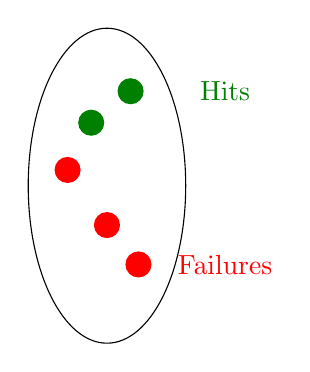
\begin{tikzpicture}
  \draw (0,0) ellipse (1 and 2); % Draw the urn

  % Define colors
  \definecolor{hitcolor}{RGB}{0,128,0} % Green for hits
  \definecolor{failcolor}{RGB}{255,0,0} % Red for failures

  % Draw the balls (adjust positions as needed)
  \node[circle, fill=hitcolor, minimum size=0.3cm] at (0.3,1.2) {};
  \node[circle, fill=hitcolor, minimum size=0.3cm] at (-0.2,0.8) {};

  \node[circle, fill=failcolor, minimum size=0.3cm] at (0,-0.5) {};
  \node[circle, fill=failcolor, minimum size=0.3cm] at (-0.5,0.2) {};
  \node[circle, fill=failcolor, minimum size=0.3cm] at (0.4,-1) {};

  % Add labels (optional)
  \node[hitcolor] at (1.5,1.2) {Hits};
  \node[failcolor] at (1.5,-1) {Failures};
\end{tikzpicture}
\end{document}
